%%%%%%%%%%%%%%%%%%%%%%%%%%%%%%%%%%%%%%%%%%%%%%%%%%%%%%%%%%%%%%%%%%%%%%%%%%%%%
%
% jape.tex
%
% hamish, 25/8/1
%
% $Id: jape.tex,v 1.49 2006/10/24 11:47:27 diana Exp $
%
%%%%%%%%%%%%%%%%%%%%%%%%%%%%%%%%%%%%%%%%%%%%%%%%%%%%%%%%%%%%%%%%%%%%%%%%%%%%%


%%%%%%%%%%%%%%%%%%%%%%%%%%%%%%%%%%%%%%%%%%%%%%%%%%%%%%%%%%%%%%%%%%%%%%%%%%%%%
\chapt[chap:jape]{JAPE: Regular Expressions over Annotations}
\markboth{JAPE: Regular Expressions over Annotations}{JAPE: Regular Expressions over Annotations}
%%%%%%%%%%%%%%%%%%%%%%%%%%%%%%%%%%%%%%%%%%%%%%%%%%%%%%%%%%%%%%%%%%%%%%%%%%%%%
\nnormalsize
%%%% qqqqqqqqqqqqqqqqqqqqqqqqq %%%%
\ifprintedbook
\else
\begin{quote}
If Osama bin Laden did not exist, it would be necessary to invent him.
For the past four years, his name has been invoked whenever
a US president has sought to increase the defence budget or wriggle out
of arms control treaties. He has been used to justify even
President Bush's missile defence programme, though neither he nor his
associates are known to possess anything approaching
ballistic missile technology. Now he has become the personification of evil
required to launch a crusade for good: the face behind the
faceless terror.

The closer you look, the weaker the case against Bin Laden becomes. While
the terrorists who inflicted Tuesday's dreadful wound
may have been inspired by him, there is, as yet, no evidence that they
were instructed by him. Bin Laden's presumed guilt appears to
rest on the supposition that he is the sort of man who would have done it.
But his culpability is irrelevant: his usefulness to western
governments lies in his power to terrify. When billions of pounds of
military spending are at stake, rogue states and terrorist warlords
become assets precisely because they are liabilities.

{\it The need for dissent}, George Monbiot, The Guardian,
Tuesday September 18, 2001.
\end{quote}
\fi
%%%% qqqqqqqqqqqqqqqqqqqqqqqqq %%%%


JAPE is a Java Annotation Patterns Engine.  JAPE provides finite state
transduction over annotations based on regular expressions.  JAPE is a
version of CPSL -- Common Pattern Specification Language\footnote{A
good description of the original version of this language is in
\htlink{http://www.ai.sri.com/\~appelt/TextPro}{\tt Doug Appelt's
TextPro manual}.  Doug was a great help to us in implementing
JAPE. Thanks Doug!}. This \chapthing\ introduces JAPE, and outlines the
functionality available. (You can find an excellent tutorial
\htlink{http://gate.ac.uk/sale/thakker-jape-tutorial/index.html}{\tt
here}; thanks to Dhaval Thakker, Taha Osmin and Phil Lakin).

JAPE allows you to recognise regular expressions in annotations on documents.
Hang on, there's something wrong here: a regular language can only describe
sets of strings, not graphs, and GATE's model of annotations is based on
graphs. Hmmm. Another way of saying this: typically, regular expressions are
applied to character strings, a simple linear sequence of items,
but here we are applying them to a much more complex data structure. The
result is that in certain cases the matching process is non-deterministic
(i.e. the results are dependent on random factors like the addresses at which
data is stored in the virtual machine): when there is structure in the graph
being matched that requires more than the power of a regular automaton to
recognise, JAPE chooses an alternative arbitrarily. However, this is not the
bad news that it seems to be, as it turns out that in many useful cases the
data stored in annotation graphs in GATE (and other language processing
systems) can be regarded as simple sequences, and matched deterministically
with regular expressions.

A JAPE grammar consists of a set of phases, each of which consists of a set of
pattern/action rules. The phases run sequentially and constitute a cascade of
finite state transducers over annotations. The left-hand-side (LHS) of the rules
consist of an annotation pattern description. The right-hand-side (RHS) consists
of annotation manipulation statements. Annotations matched on the LHS of a rule may be
referred to on the RHS by means of labels that are attached to pattern
elements. Consider the following example:

\begin{small}
\begin{verbatim}
Phase: Jobtitle
Input: Lookup
Options: control = appelt debug = true

Rule: Jobtitle1
(
 {Lookup.majorType == jobtitle} 
 (
  {Lookup.majorType == jobtitle} 
 )?
)
:jobtitle
-->
 :jobtitle.JobTitle = {rule = "JobTitle1"}
\end{verbatim}
\end{small}

The LHS is the part preceding the `\verb|-->|' and the RHS is the part following
it. The LHS specifies a pattern to be matched to the annotated GATE document, whereas the
RHS specifies what is to be done to the matched text. In this example, we have a
rule entitled `Jobtitle1', which will match text annotated with a `Lookup'
annotation with a `majorType' feature of `jobtitle', followed optionally by
further text annotated as a `Lookup' with `majorType' of `jobtitle'. Once this
rule has matched a sequence of text, the entire sequence is allocated a label by
the rule, and in this case, the label is `jobtitle'. On the RHS, we refer to this
span of text using the label given in the LHS; `jobtitle'. We say that this text
is to be given an annotation of type `JobTitle' and a `rule' feature set to
`JobTitle1'.

We began the JAPE grammar by giving it a phase name, e.g. `Phase: Jobtitle'. JAPE
grammars can be cascaded, and so each grammar is considered to be a `phase' (see
Section~\ref{sec:jape:phasesequence}). 
Phase names (and rule names) must contain only alphanumeric characters, hyphens
and underscores, and cannot start with a number.

We also provide a list of the annotation
types we will use in the grammar. In this case, we say `Input: Lookup' because
the only annotation type we use on the LHS are Lookup annotations. If no
annotations are defined, all annotations will be matched.

Then, several options are set:

\begin{itemize}

\item Control; in this case, `appelt'. This defines the method of rule matching
(see Section \ref{sec:jape:priority})

\item Debug. When set to true, if the grammar is running in Appelt
mode and there is more than one possible match, the conflicts will be
displayed on the standard output.

\end{itemize}

A wide range of functionality can be used with JAPE, making it a very powerful
system. Section~\ref{sec:jape:lhs} gives an overview of some common LHS tasks.
Section~\ref{sec:jape:operators} talks about the various operators available for
use on the LHS. After that, Section~\ref{sec:jape:rhs} outlines RHS
functionality. Section~\ref{sec:jape:priority} talks about priority and
Section~\ref{sec:jape:phasesequence} talks about phases.
Section~\ref{sec:jape:javarhs} talks about using Java code on the RHS, which is
the main way of increasing the power of the RHS. We conclude the chapter with
some miscellaneous JAPE-related topics of interest.

%%%%%%%%%%%%%%%%%%%%%%%%%%%%%%%%%%%%%%%%%%%%%%%%%%%%%%%%%%%%%%%%%%%%%%%%%%%%%
\sect[sec:jape:lhs]{The Left-Hand Side}
%%%%%%%%%%%%%%%%%%%%%%%%%%%%%%%%%%%%%%%%%%%%%%%%%%%%%%%%%%%%%%%%%%%%%%%%%%%%%

The LHS of a JAPE grammar aims to match the text span to be annotated, whilst
avoiding undesirable matches. There are various tools available to enable you
to do this. This section outlines how you would approach various common tasks
on the LHS of your JAPE grammar.

%%%%%%%%%%%%%%%%%%%%%%%%%%%%%%%%%%%%%%%%%%%%%%%%%%%%%%%%%%%%%%%%%%%%%%%%%%%%%
\subsect{Matching Entire Annotation Types}
%%%%%%%%%%%%%%%%%%%%%%%%%%%%%%%%%%%%%%%%%%%%%%%%%%%%%%%%%%%%%%%%%%%%%%%%%%%%%

The simplest pattern in JAPE is to match any single annotation of a particular
annotation type.  You can match only annotation types you specified in the
``Input'' line at the top of the file.  For example, the following will match
any Lookup annotation:

\begin{small}
\begin{verbatim}
{Lookup}
\end{verbatim}
\end{small}

If the annotation type contains anything other than ASCII letters and digits,
you need to quote it\footnote{In order for this rule to match you would also
need to quote the type in the Input line at the top of the grammar, e.g.
\texttt{Input: "html:table"}}:

\begin{small}
\begin{verbatim}
{"html:table"}
\end{verbatim}
\end{small}


%%%%%%%%%%%%%%%%%%%%%%%%%%%%%%%%%%%%%%%%%%%%%%%%%%%%%%%%%%%%%%%%%%%%%%%%%%%%%
\subsect{Using Features and Values}
%%%%%%%%%%%%%%%%%%%%%%%%%%%%%%%%%%%%%%%%%%%%%%%%%%%%%%%%%%%%%%%%%%%%%%%%%%%%%

You can specify the features (and values) of an annotation to be matched.
Several operators are supported; see Section~\ref{sec:jape:operators} for full
details:
  \begin{itemize}
  \item \verb|{Token.kind == "number"}|, \verb|{Token.length != 4}| - equality
  and inequality.
  \item \verb|{Token.string > "aardvark"}|, \verb|{Token.length < 10}| -
  comparison operators. \verb|>=| and \verb|<=| are also supported.
  \item \verb|{Token.string =~ "[Dd]ogs"}|,
  \verb|{Token.string !~ "(?i)hello"}| - regular expression.  \verb|==~| and
  \verb|!=~| are also provided, for whole-string matching.
  \item \verb|{X contains Y}|, \verb|{X notContains Y}|, \verb|{X within Y}|
  and \verb|{X notWithin Y}| for checking annotations within the context of
  other annotations.
  \end{itemize}

In the following rule, the `category' feature of the `Token' annotation is
used, along with the `equals' operator:

\begin{small}
\begin{verbatim}
Rule: Unknown
Priority: 50
( 
 {Token.category == NNP}
) 
:unknown
-->
 :unknown.Unknown = {kind = "PN", rule = Unknown}
\end{verbatim}
\end{small}

As with the annotation type, if you want to match a feature name that contains
anything other than letters or digits, it must be quoted

\begin{small}
\begin{verbatim}
 {element."xsi:type" == "xs:string"}
\end{verbatim}
\end{small}

%%%%%%%%%%%%%%%%%%%%%%%%%%%%%%%%%%%%%%%%%%%%%%%%%%%%%%%%%%%%%%%%%%%%%%%%%%%%%
\subsect[sec:jape:metaproperties]{Using Meta-Properties}
%%%%%%%%%%%%%%%%%%%%%%%%%%%%%%%%%%%%%%%%%%%%%%%%%%%%%%%%%%%%%%%%%%%%%%%%%%%%%

In addition to referencing annotation features, 
JAPE allows access to other `meta-properties' of an annotation.  This is done 
by using an `@' symbol rather than a `.' symbol after the annotation type name.
The three meta-properties that are built in are:
\begin{itemize}
\item length - returns the spanning length of the annotation.
\item string - returns the string spanned by the annotation in the document.
\item cleanString - Like string, but with extra white space stripped out.  
(i.e. `$\backslash$s+' goes to a single space and leading or trailing white 
space is removed).
\end{itemize}

\begin{small}
\begin{verbatim}
{X@length > 5}:label-->:label.New = {}
\end{verbatim}
\end{small}  

%%%%%%%%%%%%%%%%%%%%%%%%%%%%%%%%%%%%%%%%%%%%%%%%%%%%%%%%%%%%%%%%%%%%%%%%%%%%%
\subsect[sec:jape:compositionaloperators]{Building complex patterns from simple patterns}
%%%%%%%%%%%%%%%%%%%%%%%%%%%%%%%%%%%%%%%%%%%%%%%%%%%%%%%%%%%%%%%%%%%%%%%%%%%%%

So far we have seen how to build a simple pattern that matches a single
annotation, optionally with a constraint on one of its features or
meta-properties, but to do anything useful with JAPE you will need to combine
these simple patterns into more complex ones.

\subsubsect{Sequences, alternatives and grouping}

Patterns can be matched in sequence, for example:
\begin{small}
\begin{verbatim}
Rule: InLocation
(
  {Token.category == "IN"}
  {Location}
):inLoc
\end{verbatim}
\end{small}
matches a Token annotation of category ``IN'' followed by a Location
annotation.  Note that ``followed by'' in JAPE depends on the annotation types
specified in the Input line -- the above pattern matches a Token annotation and
a Location annotation provided there are no intervening annotations of a type
listed in the Input line.  The Token and Location will {\em not} necessarily be
immediately adjacent (they would probably be separated by an intervening space).
In particular the pattern would {\em not} match if ``SpaceToken'' were
specified in the Input line.

The vertical bar ``\verb!|!'' is used to denote alternatives.  For example
\begin{small}
\begin{verbatim}
Rule: InOrAdjective
(
  {Token.category == "IN"} | {Token.category == "JJ"}
):inLoc
\end{verbatim}
\end{small}
would match {\em either} a Token whose category is ``IN'' {\em or} one whose
category is ``JJ''.

Parentheses are used to group patterns:
\begin{small}
\begin{verbatim}
Rule: InLocation
(
  ({Token.category == "IN"} | {Token.category == "JJ"})
  {Location}
):inLoc
\end{verbatim}
\end{small}
matches a Token with one or other of the two category values, followed by a
Location, whereas:
\begin{small}
\begin{verbatim}
Rule: InLocation
(
  {Token.category == "IN"} |
  ( {Token.category == "JJ"}
    {Location} )
):inLoc
\end{verbatim}
\end{small}
would match either an ``IN'' Token or a sequence of ``JJ'' Token and Location.

\subsubsect{Repetition}

JAPE also provides repetition operators to allow a pattern in parentheses to be
optional (?), or to match zero or more (*), one or more (+) or some specified
number of times.  In the following example, you can see the `$\mid $' and `?'
operators being used: 
\begin{small}
\begin{verbatim}
Rule:	LocOrganization
Priority: 50

(
 ({Lookup.majorType == location} |
  {Lookup.majorType == country_adj})
{Lookup.majorType == organization}
({Lookup.majorType == organization})?
)
:orgName -->  
  :orgName.TempOrganization = {kind = "orgName", rule=LocOrganization}
\end{verbatim}
\end{small}

\subsubsect[sec:jape:ranges]{Range Notation}

Repetition ranges are specified using square brackets.
\begin{small}
\begin{verbatim}({Token})[1,3]\end{verbatim}
\end{small} matches one to three Tokens 
in a row. \begin{small}
\begin{verbatim}({Token.kind == number})[3]\end{verbatim}
\end{small} matches
exactly 3 number Tokens in a row.

%%%%%%%%%%%%%%%%%%%%%%%%%%%%%%%%%%%%%%%%%%%%%%%%%%%%%%%%%%%%%%%%%%%%%%%%%%%%%
\subsect{Matching a Simple Text String}
%%%%%%%%%%%%%%%%%%%%%%%%%%%%%%%%%%%%%%%%%%%%%%%%%%%%%%%%%%%%%%%%%%%%%%%%%%%%%

JAPE operates over annotations so it cannot match strings of text in the
document directly.  To match a string you need to match an annotation that
covers that string, typically a ``Token''.  The GATE Tokeniser adds a
``string'' feature to all the Token annotations containing the string that the
Token covers, so you can use this (or the \verb|@string| meta property) to
match text in your document.

\begin{small}
\begin{verbatim}
{Token.string == "of"}
\end{verbatim}
\end{small}

The following grammar shows a sequence of strings being matched.

\begin{small}
\begin{verbatim}
Phase:	UrlPre
Input:  Token SpaceToken
Options: control = appelt

Rule: Urlpre

(	(({Token.string == "http"}	|
	  {Token.string == "ftp"})
	 {Token.string == ":"}
	 {Token.string == "/"}
         {Token.string == "/"}
        )	|
	({Token.string == "www"}
         {Token.string == "."}
        )
):urlpre
-->
:urlpre.UrlPre = {rule = "UrlPre"}
\end{verbatim}
\end{small}

Since we are matching annotations and not text, you must be careful that the
strings you ask for are in fact single tokens.  In the example above,
\verb|{Token.string == "://"}| would never match (assuming the default ANNIE
Tokeniser) as the three characters are treated as separate tokens.

%%%%%%%%%%%%%%%%%%%%%%%%%%%%%%%%%%%%%%%%%%%%%%%%%%%%%%%%%%%%%%%%%%%%%%%%%%%%%
\subsect[sec:jape:templates]{Using Templates}
%%%%%%%%%%%%%%%%%%%%%%%%%%%%%%%%%%%%%%%%%%%%%%%%%%%%%%%%%%%%%%%%%%%%%%%%%%%%%

In cases where a grammar contains many similar or identical strings or other
literal values, JAPE supports the concept of {\it templates}.  A template is a
named value declared in the grammar file, similar to a variable in Java or
other programming languages, which can be referenced anywhere where a normal
string literal, boolean or numeric value could be used, on the left- or
right-hand side of a rule.  In the simplest case templates can be constants:
\begin{small}
\begin{verbatim}
Template: source = "Interesting entity finder"
Template: threshold = 0.6
\end{verbatim}
\end{small}
%
The templates can be used in rules by providing their names in square brackets:
\begin{small}
\begin{verbatim}
Rule: InterestingLocation
(
  {Location.score >= [threshold]}
):loc
-->
:loc.Entity = { type = Location, source = [source] }
\end{verbatim}
\end{small}
%
The JAPE grammar parser substitutes the template values for their references
when the grammar is parsed.  Thus the example rule is equivalent to
\begin{small}
\begin{verbatim}
Rule: InterestingLocation
(
  {Location.score >= 0.6}
):loc
-->
:loc.Entity = { type = Location,
  source = "Interesting entity finder" }
\end{verbatim}
\end{small}
%
The advantage of using templates is that if there are many rules in the grammar
that all reference the {\tt threshold} template then it is possible to change
the threshold for all rules by simply changing the template definition.

The name ``template'' stems from the fact that templates whose value is a
string can contain {\it parameters}, specified using \verb|${name}| notation:
\begin{small}
\begin{verbatim}
Template: url = "http://gate.ac.uk/${path}"
\end{verbatim}
\end{small}
%
When a template containing parameters is referenced, values for the parameters
may be specified:
\begin{small}
\begin{verbatim}
...
-->
:anchor.Reference = {
  page = [url path = "userguide"] }
\end{verbatim}
\end{small}
%
This is equivalent to \verb|page = "http://gate.ac.uk/userguide"|.  Multiple
parameter value assignments are separated by commas, for example:
%
\begin{small}
\begin{verbatim}
Template: proton =
  "http://proton.semanticweb.org/2005/04/proton${mod}#${n}"

...
{Lookup.class == [proton mod="km", n="Mention"]}
// equivalent to
// {Lookup.class ==
//    "http://proton.semanticweb.org/2005/04/protonkm#Mention"}
\end{verbatim}
\end{small}

The parser will report an error if a value is specified for a parameter that is
not declared by the referenced template, for example
\verb|[proton module="km"]| would not be permitted in the above example.

\subsubsect{Advanced template usage}

If a template contains parameters for which values are not provided when the
template is referenced, the parameter placeholders are passed through
unchanged.  Combined with the fact that the value for a template definition can
itself be a reference to a previously-defined template, this allows for idioms
like the following:
\begin{small}
\begin{verbatim}
Template: proton =
  "http://proton.semanticweb.org/2005/04/proton${mod}#${n}"
Template: pkm = [proton mod="km"]
Template: ptop = [proton mod="t"]

...
({Lookup.class == [ptop n="Person"]}):look
-->
:look.Mention = { class = [pkm n="Mention"], of = "Person"}
\end{verbatim}
\end{small}

(This example is inspired by the ontology-aware JAPE matching mode described in
section~\ref{sec:ontologies:ontology-aware-jape}.)

In a multi-phase JAPE grammar, templates defined in earlier phases may be
referenced in later phases.  This makes it possible to declare constants (such
as the PROTON URIs above) in one place and reference them throughout a complex
grammar.

%%%%%%%%%%%%%%%%%%%%%%%%%%%%%%%%%%%%%%%%%%%%%%%%%%%%%%%%%%%%%%%%%%%%%%%%%%%%%
\subsect{Multiple Pattern/Action Pairs}
%%%%%%%%%%%%%%%%%%%%%%%%%%%%%%%%%%%%%%%%%%%%%%%%%%%%%%%%%%%%%%%%%%%%%%%%%%%%%

It is also possible to have more than one pattern and corresponding
action, as shown in the rule below. On the LHS, each pattern is enclosed in a set
of round brackets and has a unique label; on the RHS, each label is
associated with an action. In this example, the Lookup annotation is
labelled `jobtitle' and is given the new annotation JobTitle; the
TempPerson annotation is labelled `person' and is given the new
annotation `Person'.

\begin{small}
\begin{verbatim}
Rule: PersonJobTitle
Priority: 20

(
 {Lookup.majorType == jobtitle}
):jobtitle
(
 {TempPerson}
):person
-->
    :jobtitle.JobTitle = {rule = "PersonJobTitle"},
    :person.Person = {kind = "personName", rule = "PersonJobTitle"}
\end{verbatim}
\end{small}

Similarly, labelled patterns can be nested, as in the example below,
where the whole pattern is annotated as Person, but within the
pattern, the jobtitle is annotated as JobTitle.

\begin{small}
\begin{verbatim}
Rule: PersonJobTitle2
Priority: 20

(
(
 {Lookup.majorType == jobtitle}
):jobtitle
 {TempPerson}
):person
-->
    :jobtitle.JobTitle = {rule = "PersonJobTitle"},
    :person.Person = {kind = "personName", rule = "PersonJobTitle"}
\end{verbatim}
\end{small}

%%%%%%%%%%%%%%%%%%%%%%%%%%%%%%%%%%%%%%%%%%%%%%%%%%%%%%%%%%%%%%%%%%%%%%%%%%%%%
\subsect[sec:jape:lhsmacro]{LHS Macros}
%%%%%%%%%%%%%%%%%%%%%%%%%%%%%%%%%%%%%%%%%%%%%%%%%%%%%%%%%%%%%%%%%%%%%%%%%%%%%

Macros allow you to create a definition that can then be used multiple times in
your JAPE rules. In the following JAPE grammar, we have a cascade of macros
used. The macro `AMOUNT\_NUMBER' makes use of the macros `MILLION\_BILLION' and
`NUMBER\_WORDS', and the rule `MoneyCurrencyUnit' then makes use of
`AMOUNT\_NUMBER':

\begin{small}
\begin{verbatim}
Phase: Number
Input: Token Lookup
Options: control = appelt

Macro: MILLION_BILLION
({Token.string == "m"}|
{Token.string == "million"}|
{Token.string == "b"}|
{Token.string == "billion"}|
{Token.string == "bn"}|
{Token.string == "k"}|
{Token.string == "K"}
)

Macro: NUMBER_WORDS
(
 (({Lookup.majorType == number} 
   ({Token.string == "-"})?
  )*
   {Lookup.majorType == number}
   {Token.string == "and"}
 )*
 ({Lookup.majorType == number} 
  ({Token.string == "-"})?
 )*
   {Lookup.majorType == number}
)

Macro: AMOUNT_NUMBER
(({Token.kind == number}
  (({Token.string == ","}|
    {Token.string == "."}
   )
   {Token.kind == number}
  )*
  |
  (NUMBER_WORDS)
 )
 (MILLION_BILLION)?
)

Rule: MoneyCurrencyUnit
  (        
      (AMOUNT_NUMBER)
      ({Lookup.majorType == currency_unit})
  )
:number -->
  :number.Money = {kind = "number", rule = "MoneyCurrencyUnit"}
\end{verbatim}
\end{small}

%%%%%%%%%%%%%%%%%%%%%%%%%%%%%%%%%%%%%%%%%%%%%%%%%%%%%%%%%%%%%%%%%%%%%%%%%%%%%
\subsect[sec:jape:multiconstraint]{Multi-Constraint Statements}
%%%%%%%%%%%%%%%%%%%%%%%%%%%%%%%%%%%%%%%%%%%%%%%%%%%%%%%%%%%%%%%%%%%%%%%%%%%%%

In the examples we have seen so far, most statements have contained only one
constraint. For example, in this statement, the `category' of `Token' must
equal `NNP':

\begin{small}
\begin{verbatim}
Rule: Unknown
Priority: 50
( 
 {Token.category == NNP}
) 
:unknown
-->
 :unknown.Unknown = {kind = "PN", rule = Unknown}
\end{verbatim}
\end{small}

However, it is equally acceptable to have multiple constraints in a statement.
In this example, the `majorType' of `Lookup' must be `name' {\bf and} the
`minorType' must be `surname':

\begin{small}
\begin{verbatim}
Rule: Surname
(
  {Lookup.majorType == "name",
   Lookup.minorType == "surname"}
):surname
-->
 :surname.Surname = {}
\end{verbatim}
\end{small}

Multiple constraints on the same annotation type must all be satisfied by the
{\em same} annotation in order for the pattern to match.

The constraints may refer to different annotations, and for the pattern as a
whole to match the constraints must be satisfied by annotations that
{\em start} at the same location in the document. In this example, in
addition to the constraints on the `majorType' and `minorType' of `Lookup', we
also have a constraint on the `string' of `Token':

\begin{small}
\begin{verbatim}
Rule: SurnameStartingWithDe
(
  {Token.string == "de",
   Lookup.majorType == "name",
   Lookup.minorType == "surname"}
):de
-->
 :de.Surname = {prefix = "de"}
\end{verbatim}
\end{small}

This rule would match anywhere where a Token with string `de' and a Lookup
with majorType `name' and minorType `surname' start at the same offset in
the text.  Both the Lookup and Token annotations would be included in the
\verb|:de| binding, so the Surname annotation generated would span the longer
of the two.  As before, constraints on the same annotation type must be
satisfied by a single annotation, so in this example there must be a single
Lookup matching both the major and minor types -- the rule would not match if
there were two different lookups at the same location, one of them satisfying
each constraint.

%%%%%%%%%%%%%%%%%%%%%%%%%%%%%%%%%%%%%%%%%%%%%%%%%%%%%%%%%%%%%%%%%%%%%%%%%%%%%
\subsect[sec:jape:context]{Using Context}
%%%%%%%%%%%%%%%%%%%%%%%%%%%%%%%%%%%%%%%%%%%%%%%%%%%%%%%%%%%%%%%%%%%%%%%%%%%%%

Context can be dealt with in the grammar rules in the following way.
The pattern to be annotated is always enclosed by a set of round
brackets. If preceding context is to be included in the rule, this is
placed before this set of brackets. This context is described in
exactly the same way as the pattern to be matched. If context
following the pattern needs to be included, it is placed after the
label given to the annotation. Context is used where a pattern should
only be recognised if it occurs in a certain situation, but the
context itself does not form part of the pattern to be annotated.

For example, the following rule for Time (assuming an appropriate
macro for `year') would mean that a year would only
be recognised if it occurs preceded by the words `in' or `by':

\begin{small}
\begin{verbatim}
Rule: YearContext1

({Token.string == "in"}|
 {Token.string == "by"}
)
(YEAR)
:date -->
 :date.Timex = {kind = "date", rule = "YearContext1"}
\end{verbatim}
\end{small}

Similarly, the following rule (assuming an appropriate macro for
`email') would mean that an email address would
only be recognised if it occurred inside angled brackets (which would
not themselves form part of the entity):

\begin{small}
\begin{verbatim}
Rule: Emailaddress1
({Token.string == `<'})
(
 (EMAIL)
)
:email
({Token.string == `>'})
-->
 :email.Address= {kind = "email", rule = "Emailaddress1"}
\end{verbatim}
\end{small}


It is important to remember that context is consumed by the rule, so it cannot
be reused in another rule within the same phase. So, for example, right context
for one rule cannot be used as left context for another rule.

%%%%%%%%%%%%%%%%%%%%%%%%%%%%%%%%%%%%%%%%%%%%%%%%%%%%%%%%%%%%%%%%%%%%%%%%%%%%%
\subsect[sec:jape:negation]{Negation}
%%%%%%%%%%%%%%%%%%%%%%%%%%%%%%%%%%%%%%%%%%%%%%%%%%%%%%%%%%%%%%%%%%%%%%%%%%%%%

All the examples in the preceding sections involve constraints that require the
presence of certain annotations to match.  JAPE also supports `negative'
constraints which specify the \emph{absence} of annotations.  A negative
constraint is signalled in the grammar by a `!' character.

Negative constraints are used in combination with positive ones to constrain
the locations at which the positive constraint can match.  For example:

\begin{small}
\begin{verbatim}
Rule: PossibleName
(
 {Token.orth == "upperInitial", !Lookup}
):name
-->
 :name.PossibleName = {}
\end{verbatim}
\end{small}

This rule would match any uppercase-initial Token, but only where there is no
Lookup annotation starting at the same location.  The general rule is that a
negative constraint matches at any location where the corresponding positive
constraint would \emph{not} match.  Negative constraints do not contribute any
annotations to the bindings - in the example above, the \verb|:name| binding
would contain only the Token annotation\footnote{The exception to this is when a
negative constraint is used alone, without any positive constraints in the
combination.  In this case it binds \emph{all} the annotations at the match
position that do not match the constraint.  Thus, \{!Lookup\} would bind
all the annotations starting at this location except Lookups.  In general
negative constraints should only be used in combination with positive ones.}.

Any constraint can be negated, for example:

\begin{small}
\begin{verbatim}
Rule: SurnameNotStartingWithDe
(
 {Surname, !Token.string ==~ "[Dd]e"}
):name
-->
 :name.NotDe = {}
\end{verbatim}
\end{small}

This would match any Surname annotation that does not start at the same place
as a Token with the string `de' or `De'.  Note that this is subtly different
from \verb|{Surname, Token.string !=~ "[Dd]e"}|, as the second form requires a
Token annotation to be present, whereas the first form (!Token...) will match
if there is no Token annotation at all at this location.\footnote{In the
Montreal transducer, the two forms were equivalent}

As with positive constraints, multiple negative constraints on the same
annotation type must all match the same annotation in order for the overall
pattern match to be blocked.  For example:
\begin{small}
\begin{verbatim}
{Name, !Lookup.majorType == "person", !Lookup.minorType == "female"}
\end{verbatim}
\end{small}
would match a ``Name'' annotation, but only if it does not start at the same
location as a Lookup with majorType ``person'' and minorType ``female''.  A
Lookup with majorType ``person'' and minorType ``male'' would {\em not} block
the pattern from matching.  However negated constraints on different annotation
types are independent:
\begin{small}
\begin{verbatim}
{Person, !Organization, !Location}
\end{verbatim}
\end{small}
would match a Person annotation, but only if there is no Organization
annotation {\em and} no Location annotation starting at the same place.

{\bf Note} Prior to GATE 7.0, negated constraints on the same annotation type
were considered independent, i.e. in the Name example above {\em any} Lookup of
majorType ``person'' would block the match, irrespective of its minorType.  If
you have existing grammars that depend on this behaviour you should add
\verb|negationGrouping = false| to the Options line at the top of the JAPE
phase in question.

Although JAPE provides an operator to look for the absence of a single annotation
type, there is no support for a general negative operator to prevent a rule from
firing if a particular \emph{sequence} of annotations is found. One solution to
this is to create a `negative rule' which has higher priority than the matching
`positive rule'. The style of matching must be Appelt for this to work. To create
a negative rule, simply state on the LHS of the rule the pattern that should NOT
be matched, and on the RHS do nothing. In this way, the positive rule cannot be
fired if the negative pattern matches, and vice versa, which has the same end
result as using a negative operator. A useful variation for developers is to
create a dummy annotation on the RHS of the negative rule, rather than to do
nothing, and to give the dummy annotation a rule feature. In this way, it is
obvious that the negative rule has fired. Alternatively, use Java code on the RHS
to print a message when the rule fires. An example of a matching negative and
positive rule follows. Here, we want a rule which matches a surname followed by a
comma and a set of initials. But we want to specify that the initials shouldn't
have the POS category PRP (personal pronoun). So we specify a negative rule that
will fire if the PRP category exists, thereby preventing the positive rule from
firing.
\begin{small}
\begin{verbatim}
Rule: NotPersonReverse
Priority: 20
// we don't want to match 'Jones, I'
(
 {Token.category == NNP}
 {Token.string == ","}
 {Token.category == PRP}
)
:foo
-->
{}

Rule:   PersonReverse
Priority: 5
// we want to match `Jones, F.W.'

(
 {Token.category == NNP}
 {Token.string == ","}
 (INITIALS)?
)
:person -->
\end{verbatim}
\end{small}
%

%%%%%%%%%%%%%%%%%%%%%%%%%%%%%%%%%%%%%%%%%%%%%%%%%%%%%%%%%%%%%%%%%%%%%%%%%%%%%
\subsect{Escaping Special Characters}
%%%%%%%%%%%%%%%%%%%%%%%%%%%%%%%%%%%%%%%%%%%%%%%%%%%%%%%%%%%%%%%%%%%%%%%%%%%%%

To specify a single or double quote as a
string, precede it with a backslash, e.g.
\begin{small}
\begin{verbatim}
{Token.string=="\""}
\end{verbatim}
\end{small} will match a double quote.
For other special characters, such as `\$', enclose it in double quotes, e.g.
\begin{small}
\begin{verbatim}
{Token.category == "PRP$"}
\end{verbatim}
\end{small}

%%%%%%%%%%%%%%%%%%%%%%%%%%%%%%%%%%%%%%%%%%%%%%%%%%%%%%%%%%%%%%%%%%%%%%%%%%%%%
\sect[sec:jape:operators]{LHS Operators in Detail}
\label{sec:jape:matchingoperators}
%%%%%%%%%%%%%%%%%%%%%%%%%%%%%%%%%%%%%%%%%%%%%%%%%%%%%%%%%%%%%%%%%%%%%%%%%%%%%

This section gives more detail on the behaviour of the matching operators used
on the left-hand side of JAPE rules.

Matching operators are used to specify how matching must take place between a
JAPE pattern and an annotation in the document. Equality (`==' and `!=') and
comparison (`$<$', `$<=$', `$>=$' and `$>$') operators can be used, as can
regular expression matching and contextual operators (`contains' and `within').

%%%%%%%%%%%%%%%%%%%%%%%%%%%%%%%%%%%%%%%%%%%%%%%%%%%%%%%%%%%%%%%%%%%%%%%%%%%%%
\subsect{Equality Operators}
%%%%%%%%%%%%%%%%%%%%%%%%%%%%%%%%%%%%%%%%%%%%%%%%%%%%%%%%%%%%%%%%%%%%%%%%%%%%%

The equality operators are `==' and `!='. The basic operator in JAPE is
equality. \verb|{Lookup.majorType == "person"}| matches a Lookup annotation whose
majorType feature has the value `person'. Similarly 
\verb|{Lookup.majorType != "person"}| would match any Lookup whose majorType
feature does \emph{not} have the value `person'.  If a feature is missing it is treated as if it had an
empty string as its value, so this would also match a Lookup annotation that did
not have a majorType feature at all.

Certain type coercions are performed:
\begin{itemize}
\item If the constraint's attribute is a string, it is compared with the
      annotation feature value using string equality (\verb|String.equals()|).
\item If the constraint's attribute is an integer it is treated as a
      java.lang.Long.  If the annotation feature value is also a Long, or is a
      string that can be parsed as a Long, then it is compared using
      \verb|Long.equals()|.
\item If the constraint's attribute is a floating-point number it is treated as
      a java.lang.Double.  If the annotation feature value is also a Double, or
      is a string that can be parsed as a Double, then it is compared using
      \verb|Double.equals()|.
\item If the constraint's attribute is \verb|true| or \verb|false| (without
      quotes) it is treated as a java.lang.Boolean.  If the annotation feature
      value is also a Boolean, or is a string that can be parsed as a Boolean,
      then it is compared using \verb|Boolean.equals()|.
\end{itemize}

The \verb|!=| operator matches exactly when \verb|==| doesn't.

%%%%%%%%%%%%%%%%%%%%%%%%%%%%%%%%%%%%%%%%%%%%%%%%%%%%%%%%%%%%%%%%%%%%%%%%%%%%%
\subsect{Comparison Operators}
%%%%%%%%%%%%%%%%%%%%%%%%%%%%%%%%%%%%%%%%%%%%%%%%%%%%%%%%%%%%%%%%%%%%%%%%%%%%%

The comparison operators are `$<$', `$<=$', `$>=$' and `$>$'. Comparison
operators have their expected meanings, for example \verb|{Token.length > 3}|
matches a Token annotation whose length attribute is an integer greater than 3.
The behaviour of the operators depends on the type of the constraint's attribute:

\begin{itemize}
\item If the constraint's attribute is a string it is compared with the
      annotation feature value using Unicode-lexicographic order (see
      \verb|String.compareTo()|).
\item If the constraint's attribute is an integer it is treated as a
      java.lang.Long.  If the annotation feature value is also a Long, or is a
      string that can be parsed as a Long, then it is compared using
      \verb|Long.compareTo()|.
\item If the constraint's attribute is a floating-point number it is treated as
      a java.lang.Double.  If the annotation feature value is also a Double, or
      is a string that can be parsed as a Double, then it is compared using
      \verb|Double.compareTo()|.
\end{itemize}

%%%%%%%%%%%%%%%%%%%%%%%%%%%%%%%%%%%%%%%%%%%%%%%%%%%%%%%%%%%%%%%%%%%%%%%%%%%%%
\subsect[sec:jape:operators:regex]{Regular Expression Operators}
%%%%%%%%%%%%%%%%%%%%%%%%%%%%%%%%%%%%%%%%%%%%%%%%%%%%%%%%%%%%%%%%%%%%%%%%%%%%%

The regular expression operators are `=$\sim$', `==$\sim$', `!$\sim$' and
`!=$\sim$'. These operators match regular expressions.  
\verb|{Token.string =~ "[Dd]ogs"}| matches a Token annotation whose string
feature contains a substring that matches the regular expression \verb|[Dd]ogs|, using \verb|!~| would match
if the feature value does not contain a substring that matches the regular
expression.  The \verb|==~| and \verb|!=~| operators are like \verb|=~| and
\verb|!~| respectively, but require that the \emph{whole} value match (or not
match) the regular expression\footnote{This syntax will be familiar to Groovy
users.}.  As with \verb|==|, missing features are treated as if they had the
empty string as their value, so the constraint 
\verb|{Identifier.name ==~ "(?i)[aeiou]*"}| would match an Identifier
annotation which does not have a name feature, as well as any whose name contains only vowels.

The matching uses the standard Java regular expression library, so full details
of the pattern syntax can be found in the
\htlink{http://java.sun.com/j2se/1.5.0/docs/api/java/util/regex/Pattern.html}{JavaDoc documentation for java.util.regex.Pattern}.
There are a few specific points to note:

\begin{itemize}
\item To enable flags such as case-insensitive matching you can use the
      (?\emph{flags}) notation.  See the Pattern JavaDocs for details.
\item If you need to include a double quote character in a regular expression
      you must precede it with a backslash, otherwise JAPE will give a syntax
      error.  Quoted strings in JAPE grammars also convert the sequences
      \verb|\n|, \verb|\r| and \verb|\t| to the characters newline (U+000A),
      carriage return (U+000D) and tab (U+0009) respectively, but these
      characters can match literally in regular expressions so it does not make
      any difference to the result in most cases.\footnote{However this does
      mean that it is not possible to include an n, r or t character after a
      backslash in a JAPE quoted string, or to have a backslash as the last
      character of your regular expression.  Workarounds include placing
      the backslash in a character class ([$\backslash\backslash$]|) or enabling
      the (?x) flag, which allows you to put whitespace between the backslash
      and the offending character without changing the meaning of the pattern.}
\end{itemize}

%%%%%%%%%%%%%%%%%%%%%%%%%%%%%%%%%%%%%%%%%%%%%%%%%%%%%%%%%%%%%%%%%%%%%%%%%%%%%
\subsect[sec:jape:operators:contextual]{Contextual Operators}
%%%%%%%%%%%%%%%%%%%%%%%%%%%%%%%%%%%%%%%%%%%%%%%%%%%%%%%%%%%%%%%%%%%%%%%%%%%%%

The contextual Operators are `contains' and `within', and their complements
`notContains' and `notWithin'. These operators match annotations within the
context of other annotations.

\begin{itemize}
\item contains - Written as \verb|{X contains Y}|, returns true if an 
annotation of type X completely contains an annotation of type Y.  Conversely
\verb|{X notContains Y}| matches if an annotation of type X does not contain
one of type Y.
\item within - Written as \verb|{X within Y}|, returns true if an annotation 
of type X is completely covered by an annotation of type Y.  Conversely
\verb|{X notWithin Y}| matches if an annotation of type X is not covered by an
annotation of type Y.
\end{itemize}

For any of these operators, the right-hand value (Y in the above examples) can
be a full constraint itself.  For example \verb|{X contains {Y.foo==bar}}| is
also accepted.  The operators can be used in a multi-constraint statement (see
Section~\ref{sec:jape:multiconstraint}) just like any of the traditional
ones, so \verb|{X.f1 != "something", X contains {Y.foo==bar}}| is valid.

%%%%%%%%%%%%%%%%%%%%%%%%%%%%%%%%%%%%%%%%%%%%%%%%%%%%%%%%%%%%%%%%%%%%%%%%%%%%%
\subsect[sec:jape:customoperators]{Custom Operators}
%%%%%%%%%%%%%%%%%%%%%%%%%%%%%%%%%%%%%%%%%%%%%%%%%%%%%%%%%%%%%%%%%%%%%%%%%%%%%

It is possible to add additional custom operators without modifying the JAPE
language.  There are init-time parameters to Transducer so that additional 
annotation `meta-property' accessors and custom operators can be referenced at 
runtime.  To add a custom operator, write a class that implements
gate.jape.constraint.ConstraintPredicate, make the class available to GATE
(either by putting the class in a JAR file in the \texttt{lib} directory or by
putting the class in a plugin and loading the plugin), and then list that
class name for the Transducer's `operators' property.  Similarly, to add a
custom `meta-property' accessor, write a class that implements
gate.jape.constraint.AnnotationAccessor, and then list that class name in the
Transducer's `annotationAccessors' property.

%%%%%%%%%%%%%%%%%%%%%%%%%%%%%%%%%%%%%%%%%%%%%%%%%%%%%%%%%%%%%%%%%%%%%%%%%%%%%
\sect[sec:jape:rhs]{The Right-Hand Side}
%%%%%%%%%%%%%%%%%%%%%%%%%%%%%%%%%%%%%%%%%%%%%%%%%%%%%%%%%%%%%%%%%%%%%%%%%%%%%

The RHS of the rule contains information about the annotation to be
created/manipulated. Information about the text span to be annotated is
transferred from the LHS of the rule using the label just described, and
annotated with the entity type (which follows it). Finally, attributes and their
corresponding values are added to the annotation. Alternatively, the RHS of the
rule can contain Java code to create or manipulate annotations, see
Section~\ref{sec:jape:javarhs}.

%%%%%%%%%%%%%%%%%%%%%%%%%%%%%%%%%%%%%%%%%%%%%%%%%%%%%%%%%%%%%%%%%%%%%%%%%%%%%
\subsect{A Simple Example}
%%%%%%%%%%%%%%%%%%%%%%%%%%%%%%%%%%%%%%%%%%%%%%%%%%%%%%%%%%%%%%%%%%%%%%%%%%%%%

In the simple example below, the pattern described will be
awarded an annotation of type `Enamex' (because it is an entity
name). This annotation will have the attribute `kind', with value
`location', and the attribute `rule', with value `GazLocation'. (The
purpose of the `rule' attribute is simply to ease the process of manual
rule validation).

\begin{small}
\begin{verbatim}
Rule: GazLocation
(
{Lookup.majorType == location}
)
:location -->
 :location.Enamex = {kind="location", rule=GazLocation}
\end{verbatim}
\end{small}

To create annotations whose type or features contain characters other
than ASCII letters and digits, quote them appropriately:

\begin{small}
\begin{verbatim}
 :example."New annotation" = {"entity type"="location"}
\end{verbatim}
\end{small}


%%%%%%%%%%%%%%%%%%%%%%%%%%%%%%%%%%%%%%%%%%%%%%%%%%%%%%%%%%%%%%%%%%%%%%%%%%%%%
\subsect{Copying Feature Values from the LHS to the RHS}
%%%%%%%%%%%%%%%%%%%%%%%%%%%%%%%%%%%%%%%%%%%%%%%%%%%%%%%%%%%%%%%%%%%%%%%%%%%%%
JAPE provides limited support for copying annotation feature values from the
left to the right hand side of a rule, for example:

\begin{small}
\begin{verbatim}
Rule: LocationType
(
 {Lookup.majorType == location}
):loc
-->
    :loc.Location = {rule = "LocationType", type = :loc.Lookup.minorType}
\end{verbatim}
\end{small}

This will set the `type' feature of the generated location to the value of the
`minorType' feature from the `Lookup' annotation bound to the loc label.  If
the Lookup has no minorType, the Location will have no `type' feature.  The
behaviour of {\tt newFeat = :bind.Type.oldFeat} is:
\begin{itemize}
\item Find all the annotations of type {\tt Type} from the left hand side
binding {\tt bind}.
\item Find one of them that has a non-{\tt null} value for its {\tt oldFeat}
feature (if there is more than one, which one is chosen is up to the JAPE
implementation).
\item If such a value exists, set the {\tt newFeat} feature of our newly
created annotation to this value.
\item If no such non-{\tt null} value exists, do not set the {\tt newFeat}
feature at all.
\end{itemize}
%
Notice that the behaviour is {\it deliberately underspecified} if there is more
than one {\tt Type} annotation in {\tt bind}.  If you need more control, or if
you want to copy several feature values from the same left hand side
annotation, you should consider using Java code on the right hand side of your
rule (see Section \ref{sec:jape:javarhs}).

As usual, if the annotation type or feature contains any unusual characters
then they can be quoted (\verb!type = :loc."Some annotation"."feature 2"!)

In addition to copying feature values you can also copy meta-properties (see
section~\ref{sec:jape:metaproperties}):
%
\begin{small}
\begin{verbatim}
Rule: LocationType
(
 {Lookup.majorType == location}
):loc
-->
    :loc.Location = {rule = "LocationType", text = :loc.Lookup@cleanString}
\end{verbatim}
\end{small}

The syntax ``\verb|feature = :label.AnnotationType@string|'' assigns to the
specified feature the text covered by the annotation of this type in the
binding with this label.  The \verb|@cleanString| and \verb|@length| properties
are similar.  As before, if there is more than one annotation of the given type
is bound to the same label then one of them will be chosen arbitrarily.

The ``\verb|.AnnotationType|'' may be omitted, for example
%
\begin{small}
\begin{verbatim}
Rule: LocationType
(
 {Token.category == IN}
 {Lookup.majorType == location}
):loc
-->
    :loc.InLocation = {rule = "InLoc", text = :loc@string,
                       size = :loc@length}
\end{verbatim}
\end{small}

In this case the string, cleanString or length is that covered by the whole
label, i.e. the same span as would be covered by an annotation created with
``\verb|:label.NewAnnotation = {}|''.

%%%%%%%%%%%%%%%%%%%%%%%%%%%%%%%%%%%%%%%%%%%%%%%%%%%%%%%%%%%%%%%%%%%%%%%%%%%%%
\subsect[sec:jape:optional]{Optional or Empty Labels}
%%%%%%%%%%%%%%%%%%%%%%%%%%%%%%%%%%%%%%%%%%%%%%%%%%%%%%%%%%%%%%%%%%%%%%%%%%%%%
The JAPE compiler will throw an exception if the RHS of a rule uses a label
missing from the LHS.  However, you can use labels from optional parts of the
LHS.
\begin{small}
\begin{verbatim}
Rule: NP
( (({Token.category == "DT"}):det)?
  (({Token.category ==~ "JJ.*"})*):adjs
  (({Token.category ==~ "NN.*"})+):noun
):np
-->
:det.Determiner = {},
:adjs.Adjectives = {},
:noun.Nouns = {},
:np.NP = {}
\end{verbatim}
\end{small}
%%
This rule can match a sequence consisting of only one Token whose category
feature (POS tag) starts with \verb!NN!; in this case the \verb!:det! binding is
null and the \verb!:adjs! binding is an empty annotation set, and both of them
are silently ignored when the RHS of the rule is executed.
%%%%%%%%%%%%%%%%%%%%%%%%%%%%%%%%%%%%%%%%%%%%%%%%%%%%%%%%%%%%%%%%%%%%%%%%%%%%%
\subsect{RHS Macros}
%%%%%%%%%%%%%%%%%%%%%%%%%%%%%%%%%%%%%%%%%%%%%%%%%%%%%%%%%%%%%%%%%%%%%%%%%%%%%

Macros, first introduced in the context of the left-hand side
(Section~\ref{sec:jape:lhsmacro}) can also be used on the RHS of rules. In this
case, the label (which matches the label on the LHS of the rule) should be
included in the macro.  Below we give an example of using a macro on the RHS:

\begin{small}
\begin{verbatim}
Macro: UNDERSCORES_OKAY          // separate
:match                                              // lines
{
    AnnotationSet matchedAnns = bindings.get("match");

    int begOffset = matchedAnns.firstNode().getOffset().intValue();
    int endOffset = matchedAnns.lastNode().getOffset().intValue();
    String mydocContent = doc.getContent().toString();
    String matchedString = mydocContent.substring(begOffset, endOffset);

    FeatureMap newFeatures = Factory.newFeatureMap();

    if(matchedString.equals("Spanish"))     {
     newFeatures.put("myrule",  "Lower");
    }
    else    {
     newFeatures.put("myrule",  "Upper");
    }

    newFeatures.put("quality",  "1");
    outputAS.add(matchedAnns.firstNode(), matchedAnns.lastNode(),
                              "Spanish_mark", newFeatures);
}

Rule: Lower
(
    ({Token.string == "Spanish"})
:match)-->UNDERSCORES_OKAY   // no label here, only macro name

Rule: Upper
(
    ({Token.string == "SPANISH"})
:match)-->UNDERSCORES_OKAY   // no label here, only macro name

 \end{verbatim}
\end{small}

%%%%%%%%%%%%%%%%%%%%%%%%%%%%%%%%%%%%%%%%%%%%%%%%%%%%%%%%%%%%%%%%%%%%%%%%%%%%%
\sect[sec:jape:priority]{Use of Priority}
%%%%%%%%%%%%%%%%%%%%%%%%%%%%%%%%%%%%%%%%%%%%%%%%%%%%%%%%%%%%%%%%%%%%%%%%%%%%%

Each grammar has one of 5 possible control styles: `brill', `all',
`first', `once' and `appelt'. This is specified at the beginning of the
grammar. If no control style is specified, the default is brill, but we would recommend always specifying a control style for sake of clarity.
Figure \ref{fig:jape:matching-styles} shows the different styles and how they can be interpreted.

\begin{figure}[htb]
\begin{center}
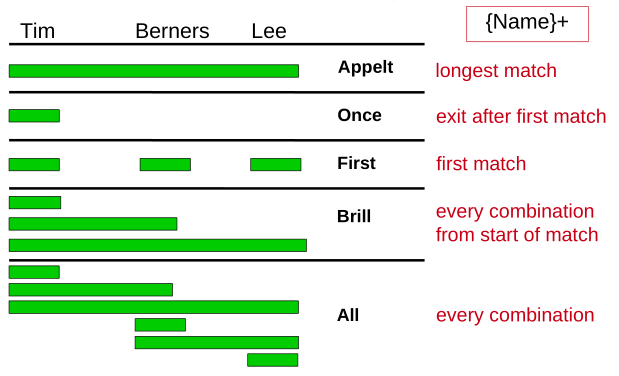
\includegraphics[scale=0.5]{jape-matching-styles.png}
\caption{JAPE Matching Styles}
\label{fig:jape:matching-styles}
\end{center}
\end{figure}

The Brill style means that when more than one rule matches the same region of
the document, they are all fired. The result of this is that a segment of text
could be allocated more than one entity type, and that no priority ordering is
necessary. Brill will execute all matching rules starting from a given position
and will advance and continue matching from the position in the document where
the longest match finishes.

The `all' style is similar to Brill, in that it will also execute all matching
rules, but the matching will continue from the next offset to the current one.

For example, where [] are annotations of type Ann
\begin{small}
\begin{verbatim}
[aaa[bbb]] [ccc[ddd]]
\end{verbatim}
\end{small}
then a rule matching \{Ann\} and creating \{Ann-2\} for the same spans will generate:
\begin{small}
\begin{verbatim}
BRILL: [aaabbb] [cccddd]
ALL: [aaa[bbb]] [ccc[ddd]]
\end{verbatim}
\end{small}

With the `first' style, a rule fires for the first match that's
found. This makes it inappropriate for rules that end in `+' or `?' or
`*'. Once a match is found the rule is fired; it does not attempt to
get a longer match (as the other two styles do).

With the `once' style, once a rule has fired, the whole JAPE phase exits after
the first match.

With the appelt style, only one rule can be fired for the same region
of text, according to a set of priority rules. Priority operates in the
following way.
%
\begin{enumerate}
\item  From all the rules that match a region of the document starting at some
point X, the one which matches the longest region is fired.
\item If more than one rule matches the same region, the one with
the highest priority is fired
\item If there is more than one rule with the same priority, the one
defined earlier in the grammar is fired.
%
\end{enumerate}

An optional priority declaration is associated with each rule, which should
be a positive integer. The higher the number, the greater the priority.
By default (if the priority declaration is missing) all rules have the
priority -1 (i.e. the lowest priority).

For example, the following two rules for location could potentially match the
same text.

\begin{small}
\begin{verbatim}
Rule:   Location1
Priority: 25

(
 ({Lookup.majorType == loc_key, Lookup.minorType == pre}
  {SpaceToken})?
 {Lookup.majorType == location}
 ({SpaceToken}
  {Lookup.majorType == loc_key, Lookup.minorType == post})?
)
:locName -->
  :locName.Location = {kind = "location", rule = "Location1"}


Rule: GazLocation
Priority: 20
  (
  ({Lookup.majorType == location}):location
  )
  -->   :location.Name = {kind = "location", rule=GazLocation}
\end{verbatim}
\end{small}

Assume we have the text `China sea', that `China'
is defined in the gazetteer as `location', and that sea is defined as
a `loc\_key' of type `post'. In this case, rule Location1 would apply,
because it matches a longer region of text starting at the same point
(`China sea', as opposed to just `China'). Now assume we just have the
text `China'. In this case, both rules could be fired, but the
priority for Location1 is highest, so it will take precedence. In this
case, since both rules produce the same annotation, so it is not so
important which rule is fired, but this is not always the case.

One important point of which to be aware is that prioritisation only
operates within a single grammar. Although we could make priority
global by having all the rules in a single grammar, this is not ideal
due to other considerations. Instead, we currently combine all the
rules for each entity type in a single grammar. An index file
(main.jape) is used to define which grammars should be used, and in
which order they should be fired.

Note also that depending on the control style, firing a rule may `consume' that
part of the text, making it unavailable to be matched by other rules. This can
be a problem for example if one rule uses context to make it more specific, and
that context is then missed by later rules, having been consumed due to use of
for example the `Brill' control style. `All', on the other hand, would allow it
to be matched.

{\bf Using priority to resolve ambiguity}

If the Appelt style of matching is selected, rule priority operates in
the following way.
\begin{enumerate}
\item
Length of rule -- a rule matching a longer pattern will fire
first.
\item
Explicit priority declaration. Use the optional Priority function to
assign a ranking. The higher the number, the higher the priority. If
no priority is stated, the default is -1.
\item
Order of rules. In the case where the above two factors do not
distinguish between two rules, the order in which the rules are stated
applies. Rules stated first have higher priority.
\end{enumerate}

Because priority can only operate within a single grammar, this can be
a problem for dealing with ambiguity issues. One solution to this is
to create a temporary set of annotations in initial grammars, and then
manipulate this temporary set in one or more later phases (for
example, by converting temporary annotations from different phases
into permanent annotations in a single final phase). See the default
set of grammars for an example of this.

If two possible ways of matching are found for the
same text string, a conflict can arise. Normally this is handled by
the priority mechanism (test length, rule priority and finally rule
precedence). If all these are equal, Jape will simply choose a match
at random and fire it. This leads ot non-deterministic behaviour,
which should be avoided.

%%%%%%%%%%%%%%%%%%%%%%%%%%%%%%%%%%%%%%%%%%%%%%%%%%%%%%%%%%%%%%%%%%%%%%%%%%%%%
\sect[sec:jape:phasesequence]{Using Phases Sequentially}
%%%%%%%%%%%%%%%%%%%%%%%%%%%%%%%%%%%%%%%%%%%%%%%%%%%%%%%%%%%%%%%%%%%%%%%%%%%%%

A JAPE grammar consists of a set of sequential phases. The list of
phases is specified (in the order in which they are to be run) in a
file, conventionally named main.jape. When loading the grammar into
GATE, it is only necessary to load this main file -- the phases will
then be loaded automatically. It is, however, possible to omit this
main file, and just load the phases individually, but this is much
more time-consuming. The grammar phases do not need to be located in
the same directory as the main file, but if they are not, the relative
path should be specified for each phase.

One of the main reasons for using a sequence of phases is that a
pattern can only be used once in each phase, but it can be reused in a
later phase. Combined with the fact that priority can only operate
within a single grammar, this can be exploited to help deal with
ambiguity issues.

The solution currently adopted is to write a grammar phase for each
annotation type, or for each combination of similar annotation types,
and to create temporary annotations. These temporary annotations are
accessed by later grammar phases, and can be manipulated as necessary
to resolve ambiguity or to merge consecutive annotations. The temporary
annotations can either be removed later, or left and simply ignored.

Generally, annotations about which we are more certain are created
earlier on. Annotations which are more dubious may be created
temporarily, and then manipulated by later phases as more information
becomes available.

An annotation generated in one phase can be referred to in a later phase, in
exactly the same way as any other kind of annotation (by specifying the name of
the annotation within curly braces). The features and values can be referred to
or omitted, as with all other annotations. Make sure that if the Input
specification is used in the grammar, that the annotation to be referred to is
included in the list.

%%%%%%%%%%%%%%%%%%%%%%%%%%%%%%%%%%%%%%%%%%%%%%%%%%%%%%%%%%%%%%%
\sect[sec:jape:javarhs]{Using Java Code on the RHS}
%%%%%%%%%%%%%%%%%%%%%%%%%%%%%%%%%%%%%%%%%%%%%%%%%%%%%%%%%%%%%%%
The RHS of a JAPE rule can consist of any Java code.
This is useful for removing temporary annotations and for percolating
and manipulating features from previous annotations. In the example below

The first rule below shows a rule which matches a first person name,
e.g. `Fred', and adds a gender feature depending on the value of the
minorType from the gazetteer list in which the name was found.
We first get the bindings associated with the person label (i.e. the
Lookup annotation). We then create a new annotation called
`personAnn' which contains this annotation, and create a new
FeatureMap to enable us to add features. Then we get the minorType
features (and its value) from the personAnn annotation (in this case,
the feature will be `gender' and the value will be `male'), and
add this value to a new feature called `gender'. We create another
feature `rule' with value `FirstName'. Finally, we add all the
features to a new annotation `FirstPerson' which attaches to the
same nodes as the original `person' binding.

Note that inputAS and outputAS represent the input and output
annotation set. Normally, these would be the same (by default when
using ANNIE, these will be the `Default' annotation set). Since the
user is at liberty to change the input and output annotation sets in
the parameters of the JAPE transducer at runtime, it cannot be
guaranteed that the input and output annotation sets will be the same,
and therefore we must specify the annotation set we are referring to.


\begin{small}
\begin{verbatim}
Rule: FirstName

(
 {Lookup.majorType == person_first}
):person
-->
{
AnnotationSet person = bindings.get("person");
Annotation personAnn = person.iterator().next();
FeatureMap features = Factory.newFeatureMap();
features.put("gender", personAnn.getFeatures().get("minorType"));
features.put("rule", "FirstName");
outputAS.add(person.firstNode(), person.lastNode(), "FirstPerson",
features);
}
\end{verbatim}
\end{small}

The second rule (contained in a subsequent grammar phase) makes use of
annotations produced by the first rule described above. Instead of
percolating the minorType from the annotation produced by the
gazetteer lookup, this time it percolates the feature from the
annotation produced by the previous grammar rule. So here it gets the
`gender' feature value from the `FirstPerson' annotation, and adds it to
a new feature (again called `gender' for convenience), which is
added to the new annotation (in outputAS) `TempPerson'. At the end of this rule,
the existing input annotations (from inputAS) are removed because they are no longer
needed. Note that in the previous rule, the existing annotations were
not removed, because it is possible they might be needed later on in
another grammar phase.


\begin{small}
\begin{verbatim}
Rule: GazPersonFirst
(
 {FirstPerson}
)
:person
-->
{
AnnotationSet person = bindings.get("person");
Annotation personAnn = person.iterator().next();
FeatureMap features = Factory.newFeatureMap();

features.put("gender", personAnn.getFeatures().get("gender"));
features.put("rule", "GazPersonFirst");
outputAS.add(person.firstNode(), person.lastNode(), "TempPerson",
features);
inputAS.removeAll(person);
}
\end{verbatim}
\end{small}

You can combine Java blocks and normal assignments (separating each block or
assignment from the next with a comma), so the above RHS could be more
simply expressed as

\begin{small}
\begin{verbatim}
-->
:person.TempPerson = { gender = :person.FirstPerson.gender,
                       rule = "GazPersonFirst" },
{
  inputAS.removeAll(bindings.get("person"));
}
\end{verbatim}
\end{small}

%%%%%%%%%%%%%%%%%%%%%%%%%%%%%%%%%%%%%%%%%%%%%
\subsect{A More Complex Example}
%%%%%%%%%%%%%%%%%%%%%%%%%%%%%%%%%%%%%%%%%%%%%

The example below is more complicated, because both the title and the
first name (if present) may have a gender feature. There is a
possibility of conflict since some first names are ambiguous, or women
are given male names (e.g. Charlie). Some titles are also ambiguous,
such as `Dr', in which case they are not marked with a gender
feature. We therefore take the gender of the title in preference to
the gender of the first name, if it is present. So, on the RHS, we
first look for the gender of the title by getting all Title
annotations which have a gender feature attached. If a gender feature
is present, we add the value of this feature to a new gender feature
on the Person annotation we are going to create. If no gender feature
is present, we look for the gender of the first name by getting all
firstPerson annotations which have a gender feature attached, and adding
the value of this feature to a new gender feature on the Person
annotation we are going to create. If there is no firstPerson
annotation and the title has no gender information, then we simply
create the Person annotation with no gender feature.

\begin{small}
\begin{verbatim}
Rule:	PersonTitle
Priority: 35
/* allows Mr. Jones, Mr Fred Jones etc. */
 
(
 (TITLE)
(FIRSTNAME | FIRSTNAMEAMBIG | INITIALS2)*
 (PREFIX)?
 {Upper}
 ({Upper})?
 (PERSONENDING)?
)
:person -->
 {
FeatureMap features = Factory.newFeatureMap();
AnnotationSet personSet = bindings.get("person");
  
// get all Title annotations that have a gender feature 
 HashSet fNames = new HashSet();
    fNames.add("gender");
    AnnotationSet personTitle = personSet.get("Title", fNames);

// if the gender feature exists
 if (personTitle != null && personTitle.size()>0)
{
  Annotation personAnn = personTitle.iterator().next();
  features.put("gender", personAnn.getFeatures().get("gender"));
}
else
{
  // get all firstPerson annotations that have a gender feature
    AnnotationSet firstPerson = personSet.get("FirstPerson", fNames);

  if (firstPerson != null && firstPerson.size()>0)
  // create a new gender feature and add the value from firstPerson
 {
  Annotation personAnn = firstPerson.iterator().next();
  features.put("gender", personAnn.getFeatures().get("gender"));
 }
}
  // create some other features
  features.put("kind", "personName");
  features.put("rule", "PersonTitle");
  // create a Person annotation and add the features we've created
outputAS.add(personSet.firstNode(), personSet.lastNode(), "TempPerson",
features);
}
\end{verbatim}
\end{small}


%%%%%%%%%%%%%%%%%%%%%%%%%%%%%%%%%%%%%%%%%%%%
\subsect[sec:jape:addingfeature]{Adding a Feature to the Document}
%%%%%%%%%%%%%%%%%%%%%%%%%%%%%%%%%%%%%%%%%%%%


This is useful when using conditional controllers, where we only want to fire
a particular resource under certain conditions. We first test the
document to see whether it fulfils these conditions or not, and attach
a feature to the document accordingly. 

In the example below, we test whether the document contains an 
annotation of type `message'. In emails, there is often an annotation
of this type (produced by the document format analysis when the
document is loaded in GATE). Note that annotations produced by
document format analysis are placed automatically in the `Original
markups' annotation set, so we must ensure that when running the
processing resource containing this grammar that we specify the
Original markups set as the input annotation set. It does not matter
what we specify as the output annotation set, because the annotation
we produce is going to be attached to the document and not to an
output annotation set. In the example, if an annotation of type
`message' is found, we add the feature `genre' with value `email' to
the document.

\begin{small}
\begin{verbatim}
 Rule: Email  
 Priority: 150  
  
 (  
  {message}  
 )  
 -->  
 {  
 doc.getFeatures().put("genre", "email");  
 } 
\end{verbatim}
\end{small}


%%%%%%%%%%%%%%%%%%%%%%%%%%%%%%%%%%%%%%%%%%%%
\subsect[sec:jape:findingtokens]{Finding the Tokens of a Matched Annotation}
%%%%%%%%%%%%%%%%%%%%%%%%%%%%%%%%%%%%%%%%%%%%

In this section we will demonstrate how by using Java on the
right-hand side one can find all Token annotations that are
covered by a matched annotation, e.g., a Person or an
Organization. This is useful if one wants to transfer some
information from the matched annotations to the tokens. For
example, to add to the Tokens a feature indicating whether or not
they are covered by a named entity annotation deduced by the
rule-based system. This feature can then be given as a feature to
a learning PR, e.g. the HMM. Similarly, one can add a feature to
all tokens saying which rule in the rule based system did the
match, the idea being that some rules might be more reliable than
others. Finally, yet another useful feature might be the length of
the coreference chain in which the matched entity is involved, if
such exists. 

The example below is one of the pre-processing JAPE grammars used
by the HMM application. To inspect all JAPE grammars, see the
muse/applications/hmm directory in the distribution.

\begin{small}
\begin{verbatim}
Phase:  NEInfo

Input: Token Organization Location Person

Options: control = appelt

Rule:   NEInfo

Priority:100

({Organization} | {Person} | {Location}):entity
-->
{
  //get the annotation set
  AnnotationSet annSet = bindings.get("entity");

  //get the only annotation from the set
  Annotation entityAnn = annSet.iterator().next();

  AnnotationSet tokenAS = inputAS.get("Token",
        entityAnn.getStartNode().getOffset(),
        entityAnn.getEndNode().getOffset());
  List<Annotation> tokens = new ArrayList<Annotation>(tokenAS);
  //if no tokens to match, do nothing
  if (tokens.isEmpty())
     return;
  Collections.sort(tokens, new gate.util.OffsetComparator());

  Annotation curToken=null;
  for (int i=0; i < tokens.size(); i++) {
    curToken = tokens.get(i);
    String ruleInfo = (String) entityAnn.getFeatures().get("rule1");
    String NMRuleInfo = (String) entityAnn.getFeatures().get("NMRule");
    if ( ruleInfo != null) {
      curToken.getFeatures().put("rule_NE_kind", entityAnn.getType());
      curToken.getFeatures().put("NE_rule_id", ruleInfo);
    }
    else if (NMRuleInfo != null) {
      curToken.getFeatures().put("rule_NE_kind", entityAnn.getType());
      curToken.getFeatures().put("NE_rule_id", "orthomatcher");
    }
    else {
      curToken.getFeatures().put("rule_NE_kind", "None");
      curToken.getFeatures().put("NE_rule_id", "None");
    }
    List matchesList = (List) entityAnn.getFeatures().get("matches");
    if (matchesList != null) {
      if (matchesList.size() == 2)
        curToken.getFeatures().put("coref_chain_length", "2");
      else if (matchesList.size() > 2 && matchesList.size() < 5)
        curToken.getFeatures().put("coref_chain_length", "3-4");
    else
        curToken.getFeatures().put("coref_chain_length", "5-more");
    }
    else
      curToken.getFeatures().put("coref_chain_length", "0");
  }//for

}

Rule:   TokenNEInfo
Priority:10
({Token}):entity
-->
{
  //get the annotation set
  AnnotationSet annSet = bindings.get("entity");

  //get the only annotation from the set
  Annotation entityAnn = annSet.iterator().next();

  entityAnn.getFeatures().put("rule_NE_kind", "None");
  entityAnn.getFeatures().put("NE_rule_id", "None");
  entityAnn.getFeatures().put("coref_chain_length", "0");
}

\end{verbatim}
\end{small}

%%%%%%%%%%%%%%%%%%%%%%%%%%%%%%%%%%%%%%%%%%%%
\subsect[sec:jape:namedjavablocks]{Using Named Blocks}
%%%%%%%%%%%%%%%%%%%%%%%%%%%%%%%%%%%%%%%%%%%%

For the common case where a Java block refers just to the annotations from a
single left-hand-side binding, JAPE provides a shorthand notation:
%
\begin{small}
\begin{verbatim}
Rule: RemoveDoneFlag

(
  {Instance.flag == "done"}
):inst
-->
:inst{
  Annotation theInstance = instAnnots.iterator().next();
  theInstance.getFeatures().remove("flag");
}
\end{verbatim}
\end{small}

This rule is equivalent to the following:
%
\begin{small}
\begin{verbatim}
Rule: RemoveDoneFlag

(
  {Instance.flag == "done"}
):inst
-->
{
  AnnotationSet instAnnots = bindings.get("inst");
  if(instAnnots != null && instAnnots.size() != 0) {
    Annotation theInstance = instAnnots.iterator().next();
    theInstance.getFeatures().remove("flag");
  }
}
\end{verbatim}
\end{small}

A label \verb|:<label>| on a Java block creates a local variable
\verb|<label>Annots| within the Java block which is the \verb|AnnotationSet|
bound to the \verb|<label>| label.  Also, the Java code in the block is only
executed if there is at least one annotation bound to the label, so you do not
need to check this condition in your own code.  Of course, if you need more
flexibility, e.g. to perform some action in the case where the label is not
bound, you will need to use an unlabelled block and perform the
\verb|bindings.get()| yourself.

%%%%%%%%%%%%%%%%%%%%%%%%%%%%%%%%%%%%%%%%%%%%
\subsect[sec:jape:javarhsoverview]{Java RHS Overview}
%%%%%%%%%%%%%%%%%%%%%%%%%%%%%%%%%%%%%%%%%%%%

When a JAPE grammar is parsed, a Jape parser creates action classes for all Java RHSs in the grammar.
(one action class per RHS) RHS Java code will be embedded as a body of the method 
\verb@doit@ and will work in context of this method. When a particular rule is fired,
the method \verb@doit@ will be executed.

Method \verb@doit@ is specified by the interface \verb@gate.jape.RhsAction@.
%% "roughly"i: do not show all details, hide what could be used in harmful ways ...
Each action class implements this interface and is generated with roughly the following template:
\begin{lstlisting}
import java.io.*;
import java.util.*;
import gate.*;
import gate.jape.*;
import gate.creole.ontology.*;
import gate.annotation.*;
import gate.util.*;
// Import: block code will be embedded here
class <AutogeneratedActionClassName>
         implements java.io.Serializable, gate.jape.RhsAction {
  private ActionContext ctx;
  public ActionContext getActionContext() { ... }
  public String ruleName() { .. }
  public String phaseName() { .. } 
    public void doit(
        gate.Document doc,
        java.util.Map<java.lang.String, gate.AnnotationSet> bindings,
        gate.AnnotationSet inputAS,
        gate.AnnotationSet outputAS,
        gate.creole.ontology.Ontology ontology) throws JapeException {
           // your RHS Java code will be embedded here ...
    }
}
\end{lstlisting}

Method \verb@doit@ has the following parameters that can be used in RHS Java
code\footnote{Prior to GATE version 8.0 there was a (deprecated) additional
parameter named \texttt{annotations} -- any grammars that used this will have
to be modified to use \texttt{inputAS} or \texttt{outputAS} as appropriate.}:
\begin{itemize}
  \item \verb@gate.Document doc@ - a document that is currently processed
  \item \verb@java.util.Map<String, AnnotationSet> bindings@ - a map of binding
    variables where a key is a (String) name of binding variable and value is
    (AnnotationSet) set of annotations corresponding to this binding
    variable\footnote{Prior to GATE 5.2 this parameter was a plain \texttt{Map}
      without type parameters, which is why you will see a lot of
      now-unnecessary casts in existing JAPE grammars such as those in ANNIE.}
  \item \verb@gate.AnnotationSet inputAS@ - input annotations
  \item \verb@gate.AnnotationSet outputAS@ - output annotations
  \item \verb@gate.creole.ontology.Ontology ontology@ - a GATE's transducer ontology
\end{itemize}

In addition, the field \texttt{ctx} provides the \texttt{ActionContext} object
to the RHS code (see the \texttt{ActionContext} JavaDoc for more).
The \texttt{ActionContext} object can be used to access the controller and 
the corpus and the name and the feature map of the processing
resource. 

In your Java RHS you can use short names for all Java classes that are
imported by the action class (plus Java classes from the packages that
are imported by default according to JVM specification: java.lang.*,
java.math.*).  But you need to use fully qualified Java class names
for all other classes. For example:

\begin{lstlisting}
-->
{
  // VALID line examples
  AnnotationSet as = ...
  InputStream is = ...
  java.util.logging.Logger myLogger =
          java.util.logging.Logger.getLogger("JAPELogger");
  java.sql.Statement stmt = ...

  // INVALID line examples
  Logger myLogger = Logger.getLogger("JapePhaseLogger");
  Statement stmt = ...
}
\end{lstlisting}

In order to add additional Java \lstinline!import! or \lstinline!import static!
statements to all Java RHS' of the rules in a JAPE grammar file, you can use
the following code at the beginning of the JAPE file:

\begin{lstlisting}
Imports: {
import java.util.logging.Logger;
import java.sql.*;
}
\end{lstlisting}

These import statements will be added to the default import statements for
each action class generated for a RHS and the corresponding classes can
be used in the RHS Java code without the need to use fully qualified names.
A useful class to know about is \lstinline!gate.Utils! (see
\htlink{http://gate.ac.uk/gate/doc/javadoc/gate/Utils.html}
{the javadoc documentation} for details), which provides static
utility methods to simplify some common tasks that are frequently used in RHS
Java code.  Adding an \lstinline!import static gate.Utils.*;! to the Imports
block allows you to use these methods without any prefix, for example:

\begin{lstlisting}
{
  AnnotationSet lookups = bindings.get("lookup");
  outputAS.add(start(lookups), end(lookups), "Person",
      featureMap("text", stringFor(doc, lookups)));
}
\end{lstlisting}

You can do the same with your own utility classes --- JAPE rules can import any
class available to GATE, including classes defined in a plugin.

The predefined methods \verb!ruleName()! and \verb!phaseName()! allow you
to easily access the rule and phase name in your Java RHS.

A JAPE file can optionally also contain Java code blocks for handling 
the events of when the controller (pipeline) running the JAPE 
processing resource
starts processing, finishes processing, or processing is aborted 
(see the JavaDoc for \texttt{ControllerAwarePR} for more information and
warnings about using this feature). 
These code blocks have to be defined after any \texttt{Import:} block
but before the first phase in the file using the \texttt{ControllerStarted:},
 \texttt{ControllerFinished:} and \texttt{ControllerAborted:} keywords:

\begin{lstlisting}
ControllerStarted: {
  // code to run when the controller starts / before any transducing is done
}
ControllerFinished: {
  // code to run right before the controller finishes / after all transducing
}
ControllerAborted: {
  // code to run when processing is aborted by an exception or by a manual
  // interruption
}
\end{lstlisting}

The Java code in each of these blocks can access the following predefined 
fields:

\begin{itemize}
  \item{\verb!controller!:} the \texttt{Controller} object running this
     JAPE transducer
  \item{\verb!corpus!:} the \texttt{Corpus} object on which this JAPE 
     transducer is run, if it is run by a \texttt{CorpusController}, 
     \texttt{null} otherwise.
  \item{\verb!ontology!:} the \texttt{Ontology} object if an Ontology LR
     has been specified as a runtime-parameter for this JAPE transducer,
     \texttt{null} otherwise
  \item{\verb!ctx!:} the \texttt{ActionContext} object. The method 
    \verb!ctx.isPREnabled()! can be used to find out if the PR is not
    disabled in a conditional controller (Note that even when a PR is disabled
    the ControllerStarted/Finished blocks are still executed!) 
  \item{\verb!throwable!:} inside the ControllerAborted block, 
     the \texttt{Throwable}
     which signalled the aborting exception
\end{itemize}

Note that these blocks are invoked even when the JAPE processing resource is
disabled in a conditional pipeline. If you want to adapt or avoid the processing
inside a block in case the processing resource is disabled, use the method
\verb=ctx.isPREnabled()= to check if the processing resource is not disabled.

%%%%%%%%%%%%%%%%%%%%%%%%%%%%%%%%%%%%%%%%%%%%%%%%%%%%%%%%%%%%%%%%%%%%%%%%%%%%%
\sect[sec:jape:speed]{Optimising for Speed}
%%%%%%%%%%%%%%%%%%%%%%%%%%%%%%%%%%%%%%%%%%%%%%%%%%%%%%%%%%%%%%%%%%%%%%%%%%%%%
%%
The way in which grammars are designed can have a huge impact on the
processing speed. Some simple tricks to keep the processing as fast as
possible are:
\begin{itemize}
%
\item avoid the use of the \texttt{*} and \texttt{+} operators. Replace them
  with range queries where possible. For example, instead of
\begin{small}
\begin{verbatim}
({Token})*
\end{verbatim}
\end{small}
 use
\begin{small}
\begin{verbatim}
({Token})[0,3]
\end{verbatim}
\end{small}
if you can predict that you won't need to recognise a
string of Tokens longer than 3.  Using \texttt{*} and \texttt{+} on very common
annotations (especially Token) is also the most common cause of out-of-memory
errors in JAPE transducers.
%
\item
avoid specifying unnecessary elements such as SpaceTokens where you
can.  To do this, use the Input specification at the beginning of the
grammar to stipulate the annotations that need to be considered. If no
Input specification is used, all annotations will be considered (so,
for example, you cannot match two tokens separated by a space unless
you specify the SpaceToken in the pattern). If, however, you specify
Tokens but not SpaceTokens in the Input, SpaceTokens do not have to be
mentioned in the pattern to be recognised. If, for example, there is
only one rule in a phase that requires SpaceTokens to be specified, it
may be judicious to move that rule to a separate phase where the
SpaceToken can be specified as Input.
%
\item
avoid the shorthand syntax for copying feature values ({\small\tt newFeat =
:bind.Type.oldFeat}), particularly if you need to copy multiple features
from the left to the right hand side of your rule.
\end{itemize}

%%%%%%%%%%%%%%%%%%%%%%%%%%%%%%%%%%%%%%%%%%%%%%%%%%%%%%%%%%%%%%%
\sect[sec:jape:ontologyaware]{Ontology Aware Grammar Transduction}
%%%%%%%%%%%%%%%%%%%%%%%%%%%%%%%%%%%%%%%%%%%%%%%%%%%%%%%%%%%%%%%
GATE supports two different methods for ontology aware grammar
transduction. Firstly it is possible to use the {\tt ontology}
feature both in grammars and annotations, while using the default
transducer. Secondly it is possible to use an ontology aware
transducer by passing an ontology language
resource to one of the subsumes methods in {\tt SimpleFeatureMapImpl}.
This second strategy does not check for ontology features, which
will make the writing of grammars easier, as there is no need to
specify {\tt ontology} when writing them. More information about
the ontology-aware transducer can be found in
Section \ref{sec:ontologies:ontology-aware-jape}.

%%%%%%%%%%%%%%%%%%%%%%%%%%%%%%%%%%%%%%%%%%%%%%%%%%%%%%%%%%%%%%%%%%%%%%%%%%%%
\sect[sec:jape:serialization]{Serializing JAPE Transducer}
%%%%%%%%%%%%%%%%%%%%%%%%%%%%%%%%%%%%%%%%%%%%%%%%%%%%%%%%%%%%%%%%%%%%%%%%%%%%%

JAPE grammars are written as files with the extension `.jape', which
are parsed and compiled at run-time to execute them over the GATE
document(s). Serialization of the JAPE Transducer adds the capability
to serialize such grammar files and use them later to bootstrap new
JAPE transducers, where they do not need the original JAPE grammar
file. This allows people to distribute the serialized version of their
grammars without disclosing the actual contents of their jape
files. This is implemented as part of the JAPE Transducer PR. The
following sections describe how to serialize and deserialize them.

\subsect{How to Serialize?}

Once an instance of a JAPE transducer is created, the option to
serialize it appears in the context menu of that instance. The context
menu can be activated by right clicking on the respective PR. Having
done so, it asks for the file name where the serialized version of the
respective JAPE grammar is stored.

\subsect{How to Use the Serialized Grammar File?}

The JAPE Transducer now also has an init-time
parameter \textit{binaryGrammarURL}, which appears as an optional
parameter to the \textit{grammarURL}. The User can use this parameter
(i.e. \textit{binaryGrammarURL}) to specify the serialized grammar
file.

%%%%%%%%%%%%%%%%%%%%%%%%%%%%%%%%%%%%%%%%%%%%%%%%%%%%%%%%%%%%%%%%%%%%%%%%%%%%
\sect[sec:jape:montrealdifferences]{Notes for Montreal Transducer Users}
%%%%%%%%%%%%%%%%%%%%%%%%%%%%%%%%%%%%%%%%%%%%%%%%%%%%%%%%%%%%%%%%%%%%%%%%%%%%

In June 2008, the standard JAPE transducer implementation gained a number of
features inspired by Luc Plamondon's `Montreal Transducer', which was available
as a GATE plugin for several years, and was made obsolete in Version 5.1. If you
have existing Montreal Transducer grammars and want to update them to work with
the standard JAPE implementation you should be aware of the following differences
in behaviour:

\begin{itemize}
\item Quantifiers (*, + and ?) in the Montreal transducer are always greedy,
      but this is not necessarily the case in standard JAPE.
\item The Montreal Transducer defines \verb|{Type.feature != value}| to be the
      same as \verb|{!Type.feature == value}| (and likewise the \verb|!~|
      operator in terms of \verb|=~|).  In standard JAPE these constructs have
      different semantics.  \verb|{Type.feature != value}| will only match if
      there is a \verb|Type| annotation whose \verb|feature| feature does not
      have the given value, and if it matches it will bind the single
      \verb|Type| annotation.  \verb|{!Type.feature == value}| will match if
      there is no \verb|Type| annotation at a given place with this feature
      (including when there is no \verb|Type| annotation at all), and if it
      matches it will bind every other annotation that starts at that location.
      If you have used \verb|!=| in your Montreal grammars and want them to
      continue to behave the same way you must change them to use the prefix-!
      form instead (see Section~\ref{sec:jape:negation}).
\item The \verb|=~| operator in standard JAPE looks for regular expression
      matches anywhere within a feature value, whereas in the Montreal
      transducer it requires the whole string to match.  To obtain the
      whole-string matching behaviour in standard JAPE, use the \verb|==~|
      operator instead (see Section~\ref{sec:jape:operators:regex}).
\end{itemize}

\sect[sec:jape:plus]{JAPE Plus}
Version $7.0$ of GATE Developer/Embedded saw the introduction of the 
\texttt{JAPE\_Plus} plugin, which includes a new JAPE execution engine, in the
form of the \texttt{JAPE-Plus Transducer}. The \texttt{JAPE-Plus Transducer}
should be a drop-in replacement for the standard JAPE Transducer: it accepts the
same language (i.e. JAPE grammars) and it has a similar set of parameters. The
\texttt{JAPE-Plus Transducer} includes a series of optimisations designed to
speed-up the execution:
\begin{description}
  \item [FSM Minimisation] the finite state machine used internally to represent
  the JAPE grammars is minimised, reducing the number of tests that to be
  performed at execution time.
  \item [Annotation Graph Indexing] JAPE Plus uses a special data structure for
  holding input annotations which is optimised for the types of tests performed
  during the execution of JAPE grammars.
  \item [Predicate Caching] JAPE pattern elements are converted into atomic
  predicates, i.e. tests that cannot be further sub-divided (such as testing if
  the value of a given annotation feature has a certain value). The truth value
  for all predicates for each input annotation is cached once calculated, using
  dynamic-programming techniques. This avoids the same test being evaluated
  multiple times for the same annotation.
  \item [Compilation of the State Machine] the finite state machine used during
  matching is converted into Java code that is then compiled on the fly. This
  allows the inlining of constants and the unwinding of execution loops.
  Additionally, the Java JIT optimisations can also apply in this set-up.
\end{description}

There are a few small differences in the behaviour of JAPE and JAPE Plus:

\begin{itemize}
  \item JAPE Plus behaves in a more deterministic fashion. There are cases where
  multiple paths inside the annotation graph can be matched with the same
  precedence, e.g. when the same JAPE rule matches different sets of annotations
  using different branches of a disjunction in the rule. In such situations, the
  standard JAPE engine will pick one of the possible paths at random and apply
  the rule using it. Separate executions of the same grammar over the same
  document can thus lead to different results. By contrast, JAPE Plus will
  always choose the same matching set of annotations. It is however not possible
  to know a priori which one will be chosen, unless the rules are re-written to
  remove the ambiguity (solution which is also possible with the standard JAPE
  engine).
  \item JAPE Plus is capable of matching zero-length annotations, i.e. 
  annotations for which the start and end offsets are the same, so they cover 
  no document text. The standard JAPE engine simply ignores such annotations,
  while JAPE Plus allows their use in rules. This can be useful in matching
  annotations converted from the original markup, for example HTML \verb!<br>! 
  tags will never have any text content.
\end{itemize}  
 
\begin{figure}[htb]
\begin{center}
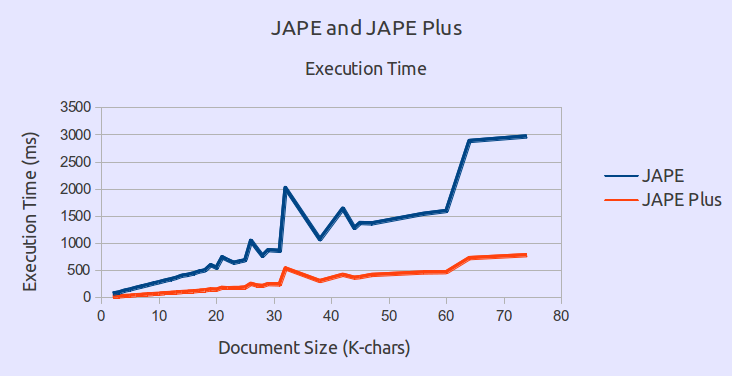
\includegraphics[scale=0.5]{jape-v-japeplus.png}
\caption{JAPE and JAPE Plus execution speed for document length}
\label{fig:jape:plus-speed}
\end{center}
\end{figure}

It is not possible to accurately quantify the speed differential between JAPE
and JAPE Plus in the general case, as that depends on the complexity of the JAPE
grammars used and of the input documents. To get one useful data point we
performed an experiment where we processed just over 8,000 web pages from the
BBC News web site, with the ANNIE NE grammars, using both JAPE and JAPE Plus. On
average the execution speed was 4 times faster when using JAPE Plus. The
smallest speed differential was 1 (i.e. JAPE Plus was as fast as JAPE), the
highest was 9 times faster. Figure~\ref{fig:jape:plus-speed} plots the execution
speed for both engines against document length. As can be seen, JAPE Plus is
consistently faster on all document sizes. 

Figure~\ref{fig:jape:plus-histogram} includes a histogram showing the number of
documents for each speed differential. For the vast majority of documents, JAPE
Plus was 3 times or more faster than JAPE.

\begin{figure}[htb]
\begin{center}
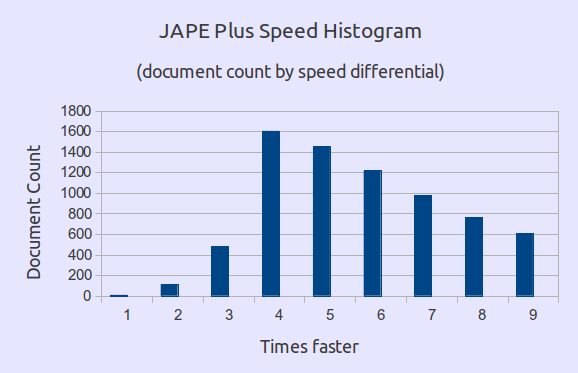
\includegraphics[scale=0.5]{jape-v-japeplus-histogram.png}
\caption{JAPE Plus execution speed differential}
\label{fig:jape:plus-histogram}
\end{center}
\end{figure}
 
